%!TEX program = xelatex
\documentclass[times,namecite]{goose-article}

\title{%
  GooseSolid/PlasticLinearElastic
}

\author{T.W.J.~de~Geus}

\contact{%
  $^*$Contact: %
  \href{mailto:tom@geus.me}{tom@geus.me} %
  \hspace{1mm}--\hspace{1mm} %
  \href{http://www.geus.me}{www.geus.me}%
  \hspace{1mm}--\hspace{1mm} %
  \href{https://github.com/tdegeus/GooseSolid}{https://github.com/tdegeus/GooseSolid}%
}

\hypersetup{pdfauthor={T.W.J. de Geus}}

\header{%
  \href{https://github.com/tdegeus/GooseSolid}{GooseSolid/PlasticLinearElastic}%
}

\newcommand\leftstar[1]{\hspace*{-.3em}~^\star\!#1}

% Former GooseFEM mat2002

\begin{document}

\maketitle

\begin{abstract}
History dependent elasto-plastic material. This corresponds to a non-linear relation between the Cauchy stress $\bm{\sigma}$ and the linear strain $\bm{\varepsilon}$, depending on the history (the accumulated plastic strain $\varepsilon_\mathrm{p}^{(t)}$, and the elastic and total strain, $\bm{\varepsilon}^{(t)}_\mathrm{e}$ and $\bm{\varepsilon}^{(t)}$). I.e.
\begin{equation*}
  \bm{\sigma} = f \left( \bm{\varepsilon} , \varepsilon_\mathrm{p}^{(t)} , \bm{\varepsilon}^{(t)}_\mathrm{e} ,\bm{\varepsilon}^{(t)} \right)
\end{equation*}
The plasticity follows power-law hardening, which is captured by the following yield stress evolution:
\begin{equation*}
  \sigma_\mathrm{y} (\varepsilon_\mathrm{p})
  = \sigma_\mathrm{y0} + \varepsilon_\mathrm{p}^m
\end{equation*}
The model is implemented in 3-D, hence it can directly be used for either 3-D or 2-D plane strain problems.
\end{abstract}

\keywords{elasto-plasticity; linear elasticity}

\setcounter{tocdepth}{2}
\tableofcontents

\vfill\newpage
\section{Constitutive model}

The model consists of the following ingredients:
%
\begin{enumerate}[(i)]
%
\item The strain, $\bm{\varepsilon}$, is additively split in an elastic part, $\bm{\varepsilon}_\mathrm{e}$, and a plastic plastic, $\bm{\varepsilon}_\mathrm{p}$. I.e.
\begin{equation}
  \bm{\varepsilon}
  = \bm{\varepsilon}_\mathrm{e}
  + \bm{\varepsilon}_\mathrm{p}
\end{equation}
%
\item The stress, $\bm{\sigma}$, is set by to the elastic strain, $\bm{\varepsilon}_\mathrm{e}$, through the following linear relation:
\begin{equation}
  \bm{\sigma}
  = \mathbb{C}_\mathrm{e} : \bm{\varepsilon}_\mathrm{e}
\end{equation}
wherein $\mathbb{C}_\mathrm{e}$ is the elastic stiffness, which reads:
\begin{align}
  \mathbb{C}_\mathrm{e}
  &= K \bm{I} \otimes \bm{I}
   + 2 G \big[ \, \mathbb{I}_\mathrm{s} - \tfrac{1}{3} \bm{I} \otimes \bm{I} \, \big]
  \\
  &= K \bm{I} \otimes \bm{I}
  + 2 G \, \mathbb{I}_\mathrm{d}
\end{align}
with $K$ and $G$ the bulk and shear modulus respectively. See Appendix~\ref{sec:ap:nomenclature} for nomenclature.
%
\item The elastic domain is bounded by the following yield function
\begin{equation}
  \Phi( \bm{\sigma} , \varepsilon_\mathrm{p} )
  = \sigma_\mathrm{eq}
  - \sigma_\mathrm{y} (\varepsilon_\mathrm{p}) \leq 0
\end{equation}
where $\sigma_\mathrm{eq}$ the equivalent stress (see Appendix~\ref{sec:ap:stress}), and $\sigma_\mathrm{y}$ the yield stress which is a non-linear function of the equivalent plastic strain $\varepsilon_\mathrm{p}$. The implementation is based on power-law hardening:
\begin{equation}
  \sigma_\mathrm{y} = \sigma_\mathrm{y0} + H \varepsilon_\mathrm{p}^m
\end{equation}
%
\item To determine the direction of plastic flow, normality is assumed. This corresponds to the following associative flow rule:
\begin{equation}
  \dot{\bm{\varepsilon}}_\mathrm{p}
  = \dot{\gamma} \bm{N}
\end{equation}
where $\dot{\gamma}$ is the plastic multiplier, and $\bm{N}$ is the Prandtl--Reuss flow vector, which is defined through normality:
\begin{equation}
  \bm{N}
  = \frac{\partial \Phi}{\partial \bm{\sigma}}
  = \frac{3}{2}
    \frac{\bm{\sigma}_\mathrm{d}}{\sigma_\mathrm{eq}}
\end{equation}
%
\item Finally, associative hardening is assumed:
\begin{equation}
  \dot{\varepsilon}_\mathrm{p}
  = \sqrt{\tfrac{2}{3} \; \dot{\bm{\varepsilon}}_\mathrm{p} : \dot{\bm{\varepsilon}}_\mathrm{p}}
  = \dot{\gamma}
\end{equation}
The equivalent plastic strain then reads
\begin{equation}
  \varepsilon_\mathrm{p} =
  \int\limits_0^t \dot{\varepsilon}_\mathrm{p} ~\mathrm{d}\tau
\end{equation}
%
\end{enumerate}
%
For a more detailed description the reader is referred to \citet[][p.\ 216-234]{DeSouzaNeto2008}.

\vfill\newpage
\section{Numerical implementation: implicit}

For the numerical implementation, first of all a numerical time integration scheme has to be selected. Here, an implicit time discretization is used, which has the favorable property of being unconditionally stable. The numerical implementation of it is done by the commonly used return-map algorithm, in which an increment in strain is first assumed fully elastic (elastic predictor). Then, if needed, a return-map is utilized to return to a physically admissible state (plastic corrector). The benefit of this scheme as that (i) the evolution of the plasticity (the state variable) can be determined by solving a single, albeit non-linear, equation; and that (ii) the linearization to obtain the consistent tangent operator is relatively straightforward.

\subsection{Elastic predictor}

Given an increment in strain
\begin{equation}
  \bm{\varepsilon}_\Delta
  = \bm{\varepsilon}^{(t+\Delta t)} - \bm{\varepsilon}^{(t)}
\end{equation}
and the state variables, evaluate the \emph{elastic trial state}:
\begin{align}
  \leftstar{\bm{\varepsilon}}_\mathrm{e}
  &= \bm{\varepsilon}_\mathrm{e}^{(t)} + \bm{\varepsilon}_\Delta
  \\
  \leftstar{\varepsilon}_\mathrm{p}
  &= \varepsilon_\mathrm{p}^{(t)}
\end{align}
The corresponding trial stress is computed by
\begin{equation}
  \leftstar{\bm{\sigma}}
  = \mathbb{C}_\mathrm{e} : \leftstar{\bm{\varepsilon}}_\mathrm{e}
\end{equation}
Finally the trial value of the yield function follows as
\begin{equation}
  \leftstar{\Phi}
  = \Phi( \leftstar{\bm{\sigma}} , \leftstar{\varepsilon}_\mathrm{p} )
  = \leftstar{\sigma}_\mathrm{eq}
  - \sigma_\mathrm{y} (\leftstar{\varepsilon}_\mathrm{p})
\end{equation}

\subsection{Trial state: elastic}

If the trial state is within the (current) yield surface, i.e.\ when
\begin{equation}
  \leftstar{\Phi} \leq 0
\end{equation}
the trial state coincides with the actual state, and:
\begin{align}
  \bm{\varepsilon}_\mathrm{e}^{(t+\Delta t)}
  &= \leftstar{\bm{\varepsilon}}_\mathrm{e}
   = \bm{\varepsilon}_\mathrm{e}^{(t)} + \bm{\varepsilon}_\Delta
  \\
  \varepsilon_\mathrm{p}^{(t+\Delta t)}
  &= \leftstar{\varepsilon}_\mathrm{p}
   = \varepsilon_\mathrm{p}^{(t)}
  \\
  \bm{\sigma}^{(t+\Delta t)}
  &= \leftstar{\bm{\sigma}}
\end{align}

Otherwise a return-map is needed (see below).

\subsection{Trial state elasto-plastic: return-map}

If the trial state is outside the (current) yield surface, i.e.\ when
\begin{equation}
  \leftstar{\Phi} > 0
\end{equation}
plastic flow occurs in the increment. A return-map is needed to return to the admissible state. The admissible state has to satisfy the following system of equations:
\begin{equation}
\begin{cases}
  \; \bm{\varepsilon}_\mathrm{e}^{(t+\Delta t)}
    &= \leftstar\bm{\varepsilon}_\mathrm{e}
     - \Delta \gamma \; \bm{N}^{(t+\Delta t)}
  \\[2mm]
  \; \varepsilon_\mathrm{p}^{(t+\Delta t)}
    &= \varepsilon_\mathrm{p}^{(t)} + \Delta \gamma
  \\[2mm]
  \; \Phi
    &= \sigma_\mathrm{eq}^{(t+\Delta t)}
     - \sigma_\mathrm{y} \big( \varepsilon_\mathrm{p}^{(t)} + \Delta\gamma \big)
     = 0
\end{cases}
\end{equation}

\subsubsection{Scalar equation return-map}

This can be reduced by using that
\begin{align}
  \bm{\sigma}_\mathrm{d}^{(t+\Delta t)}
  &= \leftstar{\bm{\sigma}}_\mathrm{d}
   - 2 G \Delta \gamma \; \bm{N}^{(t+\Delta t)}
  \\
  &= \leftstar{\bm{\sigma}}_\mathrm{d}
   - 3 G \Delta \gamma \;
   \frac{
     \bm{\sigma}_\mathrm{d}^{(t+\Delta t)}
   }{
     \sigma_\mathrm{eq}^{(t+\Delta t)}
   }
\end{align}
This implies that the trial and updated deviator stresses are \emph{co-linear}. This implies that
\begin{equation}
  \frac{\bm{\sigma}_\mathrm{d}^{(t+\Delta t)}}{\sigma_\mathrm{eq}^{(t+\Delta t)}}
  = \frac{\leftstar{\bm{\sigma}}_\mathrm{d}}{\leftstar{\sigma}_\mathrm{eq}}
  \qquad
  \text{or}
  \qquad
  \bm{N}^{(t+\Delta t)}
  = \leftstar{\bm{N}}
\end{equation}
And thus
\begin{equation}
  \bm{\sigma}_\mathrm{d}^{(t+\Delta t)}
  = \left[ 1 - \frac{3 G \Delta \gamma}{\leftstar{\sigma}_\mathrm{eq}} \right]
    \leftstar{\bm{\sigma}}_\mathrm{d}
\end{equation}
whereby the equivalent stress trivially follows as
\begin{equation}
  \sigma_\mathrm{eq}^{(t+\Delta t)} =
  \leftstar{\sigma}_\mathrm{eq} - 3 G \Delta \gamma
\end{equation}
Instead of the system return the plastic multiplier $\Delta \gamma$ can directly be found by enforcing the yield surface
\begin{equation}
\label{eq:return-scalar}
  \Phi
  = \leftstar{\sigma}_\mathrm{eq}
  - 3 G \Delta \gamma
  - \sigma_\mathrm{y} \big( \varepsilon_\mathrm{p}^{(t)} + \Delta \gamma \big)
  = 0
\end{equation}
This (non-linear) equation has to be solved for the unknown plastic multiplier $\Delta \gamma$.

\subsubsection{Linear hardening}

Linear hardening reads
\begin{equation}
  \sigma_\mathrm{y} = \sigma_\mathrm{y0} + H \varepsilon_\mathrm{p}
\end{equation}
In this case \eqref{eq:return-scalar} can be solved analytically. The solution reads
\begin{equation}
  \Delta \gamma
  = \frac{ \leftstar{\Phi} }{ 3G + H }
\end{equation}

\subsubsection{Non-linear hardening}

\begin{enumerate}[(1)]
%
\item Initial guess:
\begin{equation}
  \Delta \gamma
    := 0
\end{equation}
and evaluate
\begin{equation}
  \tilde{\Phi}
    := \leftstar{\Phi}
\end{equation}
%
\item Perform Newton-Raphson iteration:
%
\begin{itemize}
%
\item Hardening slope
\begin{equation}
  H
  := \left.
     \frac{
       \mathrm{d} \sigma_\mathrm{y}
     }{
       \mathrm{d} \varepsilon_\mathrm{p}
     }
     \right|_{\varepsilon_\mathrm{p}^{(t)} + \Delta \gamma}
\end{equation}
%
\item Residual derivative:
\begin{equation}
  d := \frac{\mathrm{d} \tilde{\Phi}}{\mathrm{d} \Delta \gamma}
     = -3G - H
\end{equation}
%
\item Update guess for the plastic multiplier:
\begin{equation}
  \Delta \gamma := \Delta \gamma - \frac{\tilde{\Phi}}{d}
\end{equation}
%
\end{itemize}
%
\item Check for convergence:
\begin{equation}
\tilde{\Phi}
  := \leftstar{\sigma}_\mathrm{eq}
   - 3 G \Delta \gamma
   - \sigma_\mathrm{y} ( \varepsilon_\mathrm{p}^{(t)} + \Delta \gamma )
\end{equation}
Stop if:
\begin{equation}
  \big| \tilde{\Phi} \big| \leq \epsilon_\mathrm{tol}
\end{equation}
Otherwise continue with (2)
%
\end{enumerate}

\subsubsection{Trial state update}

Finally, the trial state is updated:
\begin{itemize}
%
\item The updated stress tensor
\begin{equation}
  \bm{\sigma}^{(t+\Delta t)}
    = \sigma_\mathrm{m}^{(t+\Delta t)} \bm{I}
    + \bm{\sigma}_\mathrm{d}^{(t+\Delta t)}
\end{equation}
with
\begin{align}
  \sigma_\mathrm{m}^{(t+\Delta t)}
    &= \leftstar{\sigma}_\mathrm{m}
  \\
  \bm{\sigma}_\mathrm{d}^{(t+\Delta t)}
    &= \left(
         1 - \frac{3 G \Delta \gamma}{\leftstar{\sigma}_\mathrm{eq}}
       \right) \leftstar{\bm{\sigma}}_\mathrm{d}
\end{align}
%
\item The updated elastic strain tensor
\begin{equation}
  \bm{\varepsilon}_\mathrm{e}^{(t+\Delta t)}
    = \frac{1}{2G} \bm{\sigma}^{(t+\Delta t)}_\mathrm{d}
    + \tfrac{1}{3} \;\mathrm{tr} (\leftstar{\bm{\varepsilon}}) \bm{I}
\end{equation}
%
\item The updated equivalent plastic strain:
\begin{equation}
  \varepsilon_\mathrm{p}^{(t+\Delta t)}
    = \varepsilon_\mathrm{p}^{(t)}
    + \Delta \gamma
\end{equation}
%
\end{itemize}

\section{Consistent tangent}

The consistent tangent, denoted using $\mathbb{C}_\mathrm{ep}$ below, is dependent on whether the trial state is elastic or whether it is plastic.
\begin{itemize}
%
\item In the case that the trial is elastic (i.e.\ $\leftstar{\Phi} \leq 0$), the relationship between stress and strain is linear. Specifically
\begin{equation}
  \bm{\sigma}^{(t+\Delta t)}
    = \leftstar{\bm{\sigma}}
    = \mathbb{C}_\mathrm{e} : \leftstar{\bm{\varepsilon}}_\mathrm{e}
    = \mathbb{C}_\mathrm{e} : \bm{\varepsilon}^{(t+\Delta t)}
\end{equation}
The tangent then trivially follows:
\begin{equation}
  \mathbb{C}_\mathrm{ep}
  =
  \frac{
    \partial  \bm{\sigma}^{(t+\Delta t)} \hfill
  }{
    \partial \bm{\varepsilon}^{(t+\Delta t)} \hfill
  }
  =
  \mathbb{C}_\mathrm{e}
\end{equation}
%
\item In the case that the trial is plastic (i.e.\ $\leftstar{\Phi} > 0$)
The tangent can now be obtained by
\begin{equation}
  \mathbb{C}_\mathrm{ep}
  =
  \frac{
    \partial  \bm{\sigma}^{(t+\Delta t)} \hfill
  }{
    \partial \bm{\varepsilon}^{(t+\Delta t)} \hfill
  }
  =
  \frac{
    \partial ~\bm{\sigma}^{(t+\Delta t)} \hfill
  }{
    \partial \;\leftstar{\bm{\varepsilon}}_\mathrm{e} \hfill
  }
  :
  \frac{
    \partial \;\leftstar{\bm{\varepsilon}}_\mathrm{e} \hfill
  }{
    \partial ~\bm{\varepsilon}^{(t+\Delta t)}
  }
  =
  \frac{
    \partial ~\bm{\sigma}^{(t+\Delta t)} \hfill
  }{
    \partial \;\leftstar{\bm{\varepsilon}}_\mathrm{e} \hfill
  }
  :
  \mathbb{I}
  =
  \frac{
    \partial ~\bm{\sigma}^{(t+\Delta t)} \hfill
  }{
    \partial \;\leftstar{\bm{\varepsilon}}_\mathrm{e} \hfill
  }
\end{equation}
The result reads as follows (see derivation below)
\begin{equation}
  \mathbb{C}_\mathrm{ep}
  =
  \mathbb{C}_\mathrm{e} -
  \frac{6 G^2 \Delta \gamma}{\leftstar{\sigma}_\mathrm{eq}}
  \mathbb{I}_\mathrm{d}
  + 4 G^2
  \left[
    \frac{\Delta \gamma}{\leftstar{\sigma}_\mathrm{eq}} -
    \frac{1}{3 G + H}
  \right]
  \leftstar{\bm{N}} \otimes \leftstar{\bm{N}}
\end{equation}
%
\end{itemize}

\subsection*{Derivation}

We begin by writing an explicit, linear, relation between the actual stress $\bm{\sigma}^{(t+\Delta t)}$ and the trial elastic strain $\leftstar{\bm{\varepsilon}}_\mathrm{e}$, as follows
\begin{align}
  \bm{\sigma}^{(t+\Delta t)}
    &= \sigma_\mathrm{m}^{(t+\Delta t)} \bm{I}
     + \bm{\sigma}_\mathrm{d}^{(t+\Delta t)}
    \\
    &= \leftstar{\sigma}_\mathrm{m} \bm{I}
    + \left( 1- \frac{3 G \Delta \gamma}{\leftstar{\sigma}_\mathrm{eq}} \right)
      \leftstar{\bm{\sigma}}_\mathrm{d}
    \\
    &= \leftstar{\sigma}_\mathrm{m} \bm{I}
     + \left( 1-\frac{3 G \Delta\gamma}{\leftstar{\sigma}_\mathrm{eq}} \right)
       2 G \; \leftstar{\bm{\varepsilon}}_\mathrm{e}^\mathrm{d}
    \\
    &=
    \left[
      \mathbb{C}_\mathrm{e} -
      \frac{6 G^2 \Delta \gamma}{\leftstar{\sigma}_\mathrm{eq}} \, \mathbb{I}_\mathrm{d}
    \right] : \leftstar{\bm{\varepsilon}}_\mathrm{e}
\end{align}
Partial differentiation of this reads
\begin{align}
\frac{
  \partial ~\bm{\sigma}^{(t+\Delta t)} \hfill
}{
  \partial \;\leftstar{\bm{\varepsilon}}_\mathrm{e} \hfill
} =
\mathbb{C}_\mathrm{e}
- \frac{6 G^2 \Delta \gamma}{\leftstar{\sigma}_\mathrm{eq}} \mathbb{I}^d
- \frac{6 G^2}{\leftstar{\sigma}_\mathrm{eq}} \;
\left( \frac{
  \partial ~\Delta \gamma \hfill
}{
  \partial \;\leftstar{\bm{\varepsilon}}_\mathrm{e} \hfill
} \right) \otimes
(\leftstar{\bm{\varepsilon}}_\mathrm{e})_\mathrm{d}
+ \frac{6 G^2 \Delta \gamma}{\leftstar{\sigma}_\mathrm{eq}^2} \;
\left( \frac{
  \partial \;\leftstar{\sigma}_\mathrm{eq} \hfill
}{
  \partial \;\leftstar{\bm{\varepsilon}}_\mathrm{e} \hfill
} \right) \otimes
(\leftstar{\bm{\varepsilon}}_\mathrm{e})_\mathrm{d}
\end{align}
For which the following is needed:
\begin{itemize}
%
\item Equivalent stress
\begin{equation}
  \frac{\partial \sigma_\mathrm{eq} \hfill}{\partial \bm{\sigma} \hfill}
  = \frac{\partial \sigma_\mathrm{eq} \hfill}{\partial \bm{\sigma}_\mathrm{d} \hfill}
  = \frac{\partial}{\partial \bm{\sigma}_\mathrm{d} } \left( \sqrt{ \tfrac{3}{2} \bm{\sigma}_\mathrm{d} : \bm{\sigma}_\mathrm{d} } \right)
  = \frac{1}{2 \sigma_\mathrm{eq} } \frac{\partial}{\partial \bm{\sigma}_\mathrm{d}} \left( \tfrac{3}{2} \bm{\sigma}_\mathrm{d} : \bm{\sigma}_\mathrm{d} \right)
  = \frac{3}{2} \frac{\bm{\sigma}_\mathrm{d}}{\sigma_\mathrm{eq}} = \bm{N} = \leftstar{\bm{N}}
\end{equation}
hence:
\begin{equation}
  \frac{
    \partial \;\leftstar{\sigma}_\mathrm{eq} \hfill
  }{
    \partial \;\leftstar{\bm{\varepsilon}}_\mathrm{e} \hfill
  } =
  2 G \, \leftstar{\bm{N}}
\end{equation}
%
\item Plastic multiplier
\begin{align}
  \frac{
    \partial ~\Delta \gamma \hfill
  }{
    \partial \;\leftstar{\bm{\varepsilon}}_\mathrm{e}  \hfill
  }
  =
  \left( \frac{
    \partial ~\Delta \gamma \hfill
  }{
    \partial ~\Phi \hfill
  } \right) \;
  \left( \frac{
    \partial \,~\Phi \hfill
  }{
    \partial \,\leftstar{\sigma}_\mathrm{eq} \hfill
  } \right) \;
  \left( \frac{
    \partial \,\leftstar{\sigma}_\mathrm{eq} \hfill
  }{
    \partial \,\leftstar{\bm{\varepsilon}}_\mathrm{e} \hfill
  } \right) \;
  &= \frac{2 G}{3 G + H} \, \leftstar{\bm{N}}
\end{align}
%
\end{itemize}

\vfill\newpage
\section{Examples}

\subsection{Linear vs.\ non-linear hardening}

In this example we consider a material point subject to simple shear deformation
\begin{equation}
  \bm{\varepsilon}(t) = \gamma(t) \left[ \vec{e}_x \vec{e}_y + \vec{e}_y \vec{e}_x \right]
\end{equation}
The response is a stress of the form
\begin{equation}
  \bm{\sigma}(t) = \tau(t) \left[ \vec{e}_x \vec{e}_y + \vec{e}_y \vec{e}_x \right]
\end{equation}
For a specific set of parameters response is shown in Figure~\ref{eq:powerlaw}. Notice that a  normalization factor has been introduced such that the values along the axis are those of the equivalent stress $\sigma_\mathrm{eq} = \tau \sqrt{3}$.

\begin{figure}[htp]
  \centering
  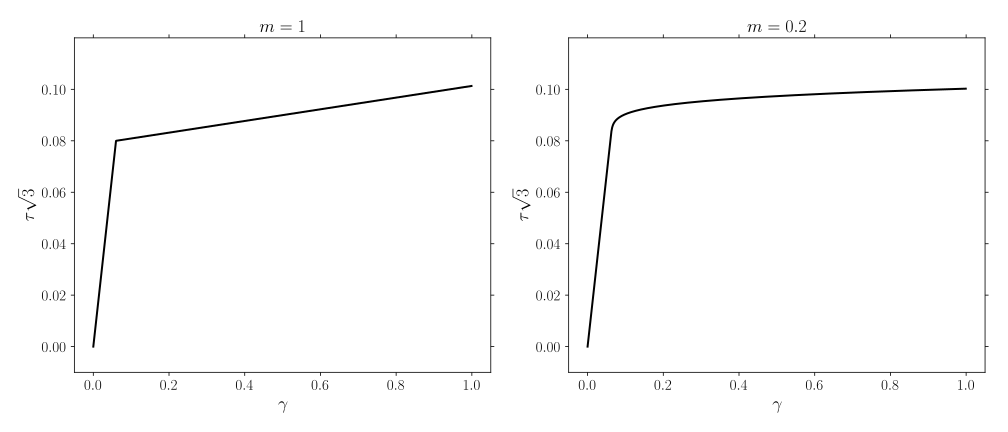
\includegraphics[width=1.\textwidth]{example}
  \caption{Linear vs.\ power-law hardening}
  \label{eq:powerlaw}
\end{figure}


\appendix
\vfill\newpage

\section{Nomenclature}
\label{sec:ap:nomenclature}


\begin{itemize}
%
\item Dyadic tensor product
\begin{align}
  \mathbb{C} &= \bm{A} \otimes \bm{B} \\
  C_{ijkl}   &= A_{ij} \,      B_{kl}
\end{align}
%
\item Double tensor contraction
\begin{align}
  C &= \bm{A} : \bm{B} \\
    &= A_{ij} \, B_{ji}
\end{align}
%
\item Deviatoric projection tensor
%
\begin{equation}
  \mathbb{I}_\mathrm{d}
  = \mathbb{I}_\mathrm{s} - \tfrac{1}{3} \bm{I} \otimes \bm{I}
\end{equation}
%
\end{itemize}


\section{Stress measures}
\label{sec:ap:stress}


\begin{itemize}
%
\item Mean stress
%
\begin{equation}
\sigma_\mathrm{m}
= \tfrac{1}{3} \, \mathrm{tr} ( \bm{\sigma} )
= \tfrac{1}{3} \, \bm{\sigma} : \bm{I}
\end{equation}
%
\item Stress deviator
%
\begin{equation}
  \bm{\sigma}_\mathrm{d}
  = \bm{\sigma} - \sigma_\mathrm{m} \, \bm{I}
  = \mathbb{I}_\mathrm{d} : \bm{\sigma}
\end{equation}
%
\item Von Mises equivalent stress
\begin{align}
\sigma_\mathrm{eq}
= \sqrt{ \tfrac{3}{2} \, \bm{\sigma}_\mathrm{d} : \bm{\sigma}_\mathrm{d} }
= \sqrt{ 3 J_2(\bm{\sigma}) }
\end{align}
where the second-stress invariant
\begin{align}
J_2 = \tfrac{1}{2} \, || \, \bm{\sigma}_\mathrm{d} \, ||^2
    = \tfrac{1}{2} \, \bm{\sigma}_\mathrm{d} : \bm{\sigma}_\mathrm{d}
\end{align}
%
\end{itemize}

\bibliography{library}

\end{document}
